\documentclass[prl,twocolumn,amsmath,amssymb,superscriptaddress]{revtex4-2}

\usepackage{graphicx}
\usepackage{verbatim}
\usepackage{braket}
\usepackage{epsfig}
\usepackage{epstopdf}
\usepackage{amsfonts}
\usepackage{amsthm}
\usepackage{amsmath}
\usepackage{amssymb}
\usepackage{color}
\usepackage[usenames,dvipsnames,svgnames,table]{xcolor}
\usepackage{hyperref}
\hypersetup{colorlinks=true,linkcolor=NavyBlue,citecolor=BrickRed,urlcolor=NavyBlue}
\usepackage{dsfont}
\usepackage{color}
\usepackage{grffile}
\usepackage{bm}
\usepackage{lipsum}
%end of packages

\begin{document}

\title{PHY180: Pendulum Project}
\author{Luyu Wu Vankerkwijk}
\date{\today}


\maketitle

\section{Introduction}
The simple pendulum is a common system in physics education. However, hiding in it's motion is a complicated non-linear problem---unlike the simplified harmonic motion equation we are often offered.

This paper investigates the non-linear behaviors of a pendulum, largely through experimental analysis, and correlates the findings to an offered linear model of the pendulum:

\begin{equation}
    \theta(t) = \theta_0e^{-t/\tau}cos\left(\frac{2\pi t}{T}+\phi_0\right)
\end{equation}

This equation (Wilson, 2025) defines the angle of the pendulum as a function of time, where $\theta_0$ and $\phi_0$ are initial conditions, and $\tau$ a constant damping factor.


Experiments were performed using a home-built pendulum, tracked using a high-speed camera. Data was processed to determine experimental relationships between amplitude-period, amplitude-damping, as well as length-period and length-damping were investigated.

\section{Experimental Methods}
The experimental setup consists of a 3 m wool string, wrapped around a cloth hanger attached to a nook in the wall. A cloth hanger is used such that the string can be spooled as to control the length of the pendulum.

The top of the string is bound in such a way that the position of the end of the pendulum does not change. At the bottom of the pendulum, a metal mass with a ring soldered onto it is bound. The mass of the pendulum blob is 54 grams while the full strings is roughly 2 grams. A strand length of $74.5 cm \pm 0.05 cm$ was used in trials where length was kept constant. Note that effective length is affected by the length of boundary and blob.

\begin{figure}[htb]
    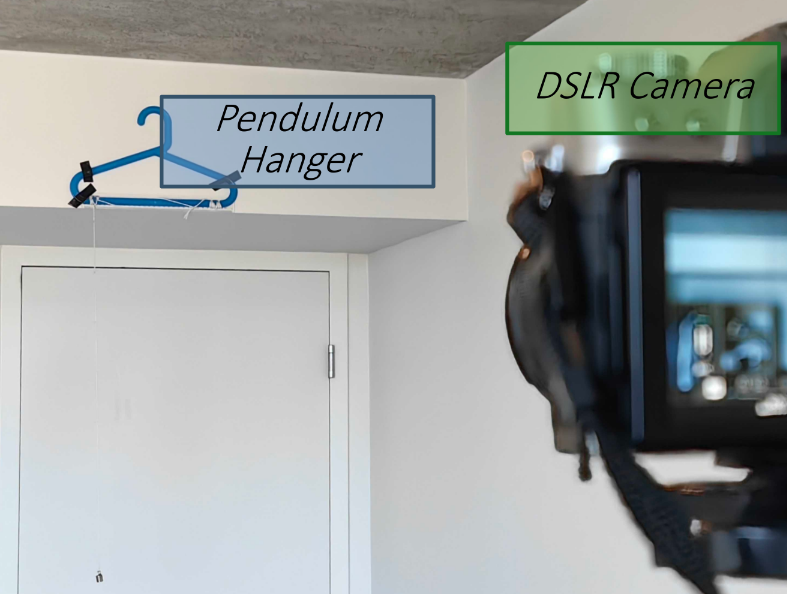
\includegraphics[width=0.6\linewidth]{setup.png}
    \caption{Picture of experimental setup.}
    \label{fig:experiment_setup}
\end{figure}

\newpage

The pendulum system was recorded from approximately 4 meters away (so as to minimize parallax) using a DSLR camera. A shutter speed of $1/1000$ and motion FPS of $60$ were used so as to minimize motion blurring, and maintain a high time resolution.

The pendulum was carefully released by hand, and trials with qualitatively significant out-of-plane movement were rejected (see Appendix B).



\begin{figure}[htb]
    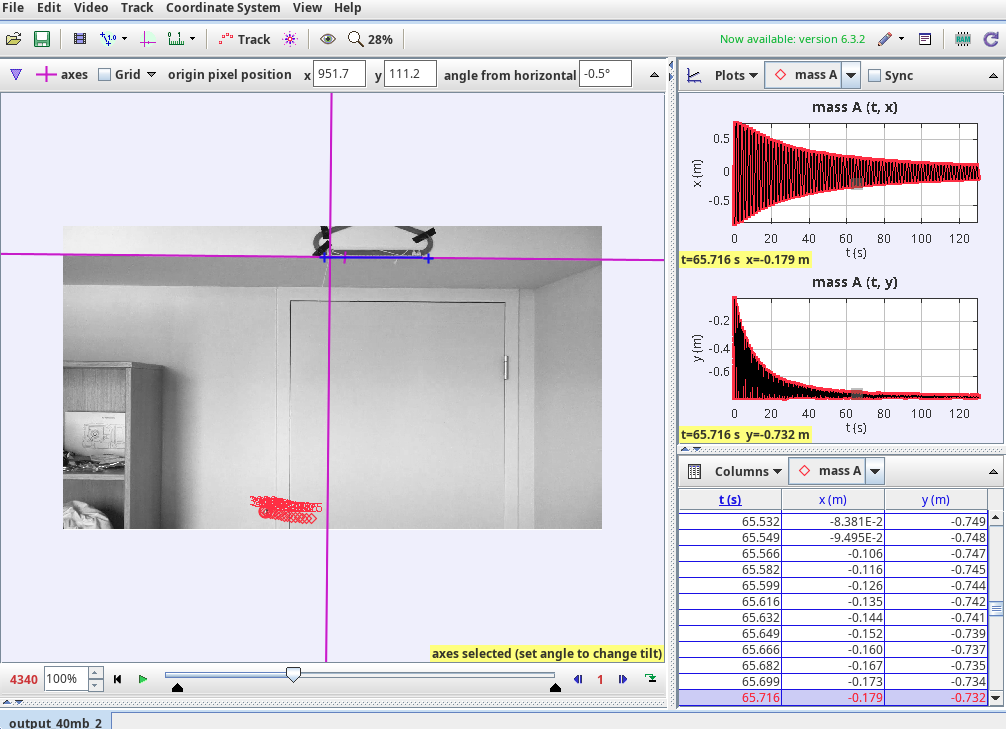
\includegraphics[width=0.7\linewidth]{tracker.png}
    \caption{OSP Tracker software used to obtain projected pendulum position as a function of time.}
    \label{fig:tracker}
\end{figure}

All data was processed in a custom Python script (Appendix A). In processing the data, we assume that the motion of the pendulum is continuous in reality (non-linear interpolation between points) so as to achieve better time resolution.

SciPy peak detection was performed. Exact periods were performed by iterating through adjascent peak points and finding the time difference (then repeated for the bottom peaks).
\newpage
\section{Results}

\begin{figure}[htb]
    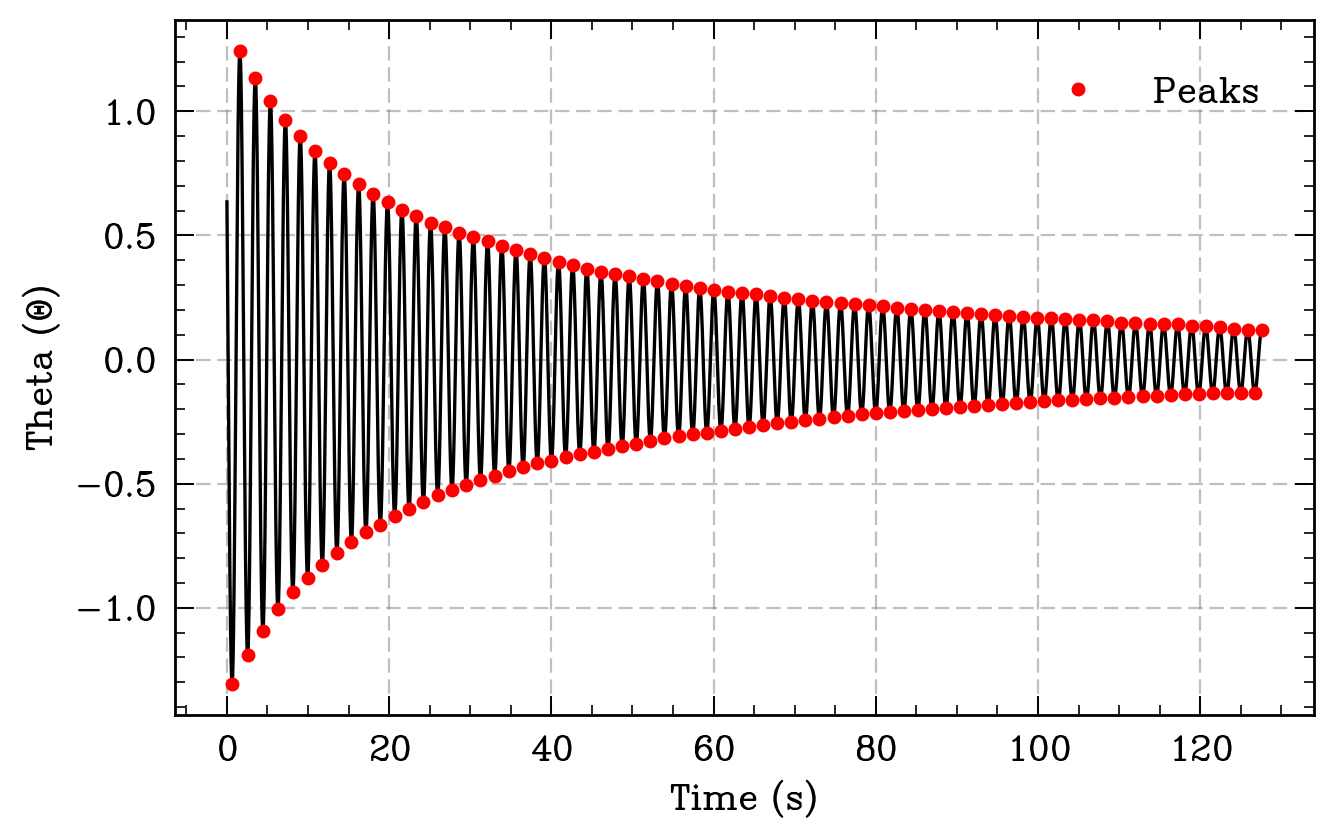
\includegraphics[width=1\linewidth]{angle_time.png}
    \label{fig:angle_time}
    \caption{Plot of pendulum angle against time ($t=0$ being arbitrary). Peaks are found using interpolative smoothing as mentioned in \textbf{Procedure}.}
\end{figure}

\subsection{Period Non-Linearity}

\begin{figure}[htb]
    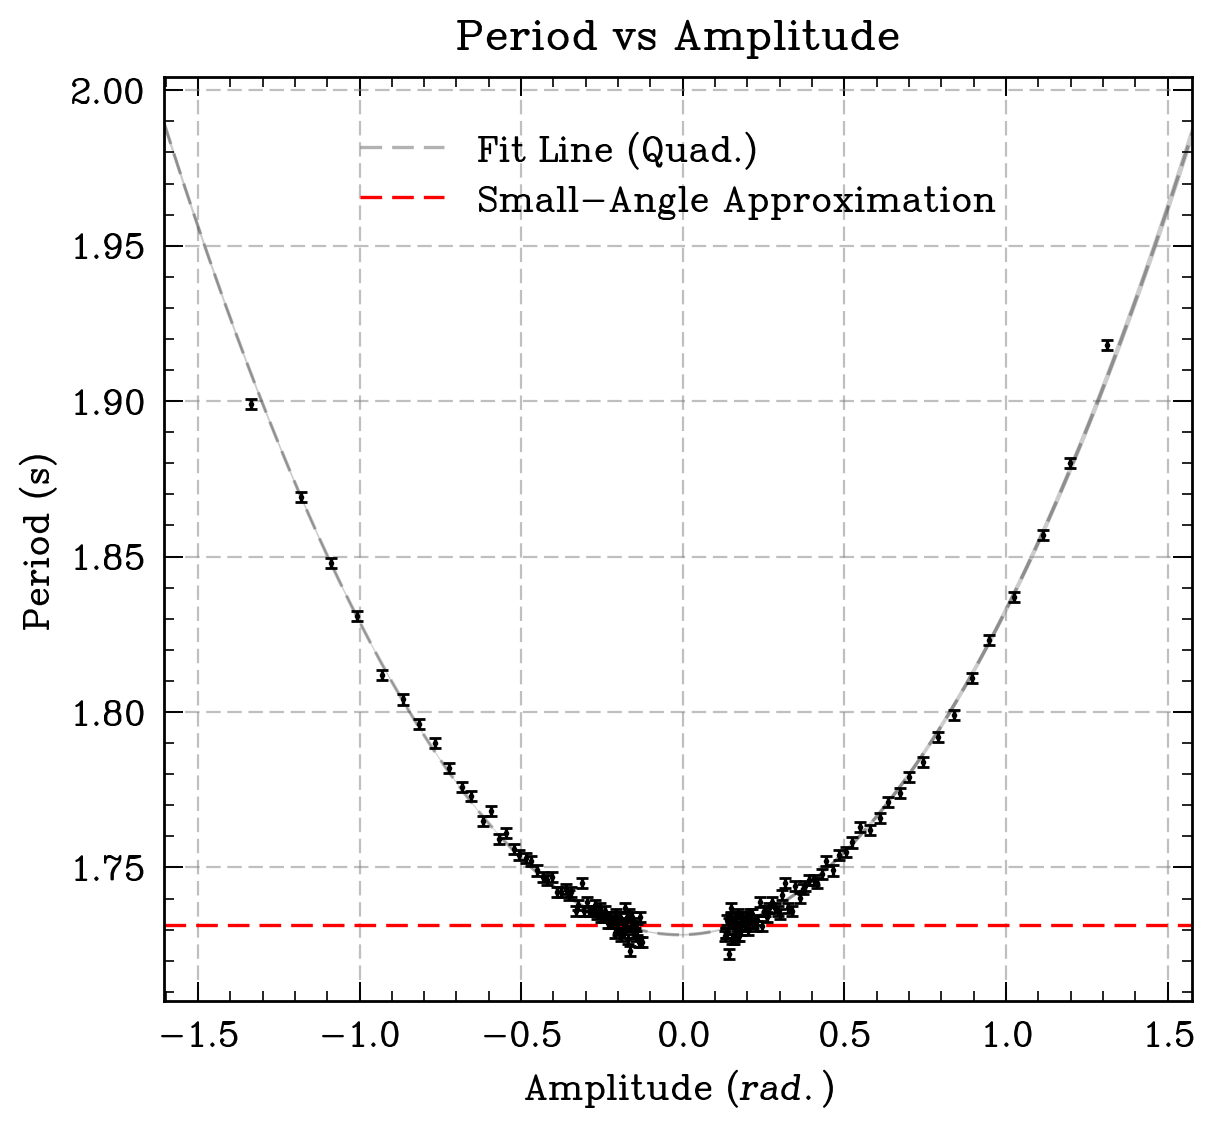
\includegraphics[width=1\linewidth]{amp-per.png}
    \label{fig:amplitude-period}
    \caption{Plot of pendulum period against oscillation amplitude. Datapoint errorbars are calculated using standard deviation ($\epsilon = 1\sigma$). $\theta$ referenced in the legend is the transient amplitude of oscillation.}
\end{figure}



\subsection{Damping Factor}


\begin{figure}[htb]
    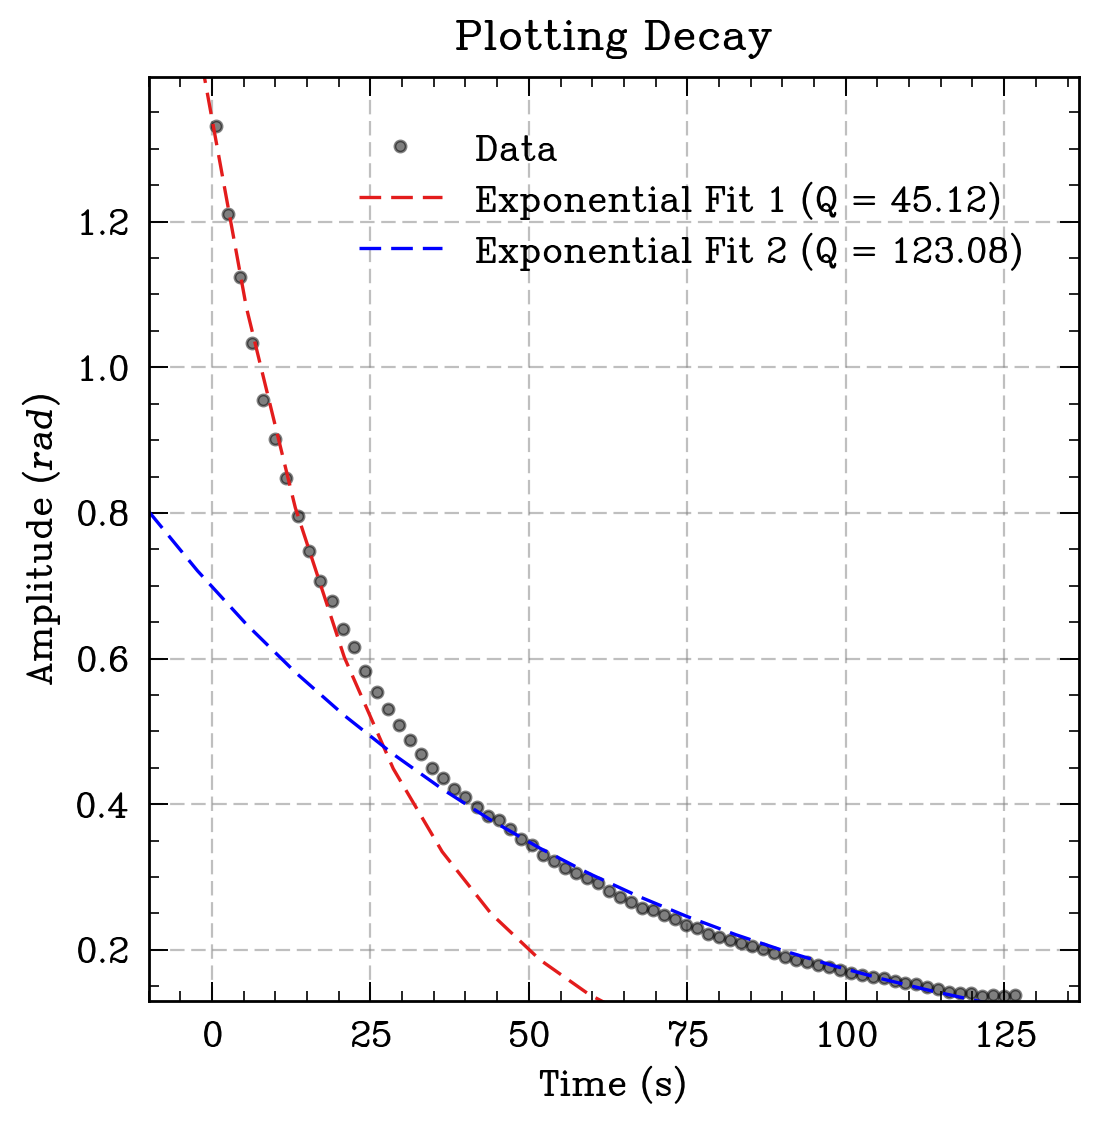
\includegraphics[width=0.8\linewidth]{decay.png}
    \label{fig:decay}
    \caption{Plot of pendulum period against oscillation amplitude. Datapoint errorbars are calculated using standard deviation ($\epsilon = 1\sigma$). $\theta$ referenced in the legend is the transient amplitude of oscillation.}
\end{figure}

\begin{figure}[htb]
    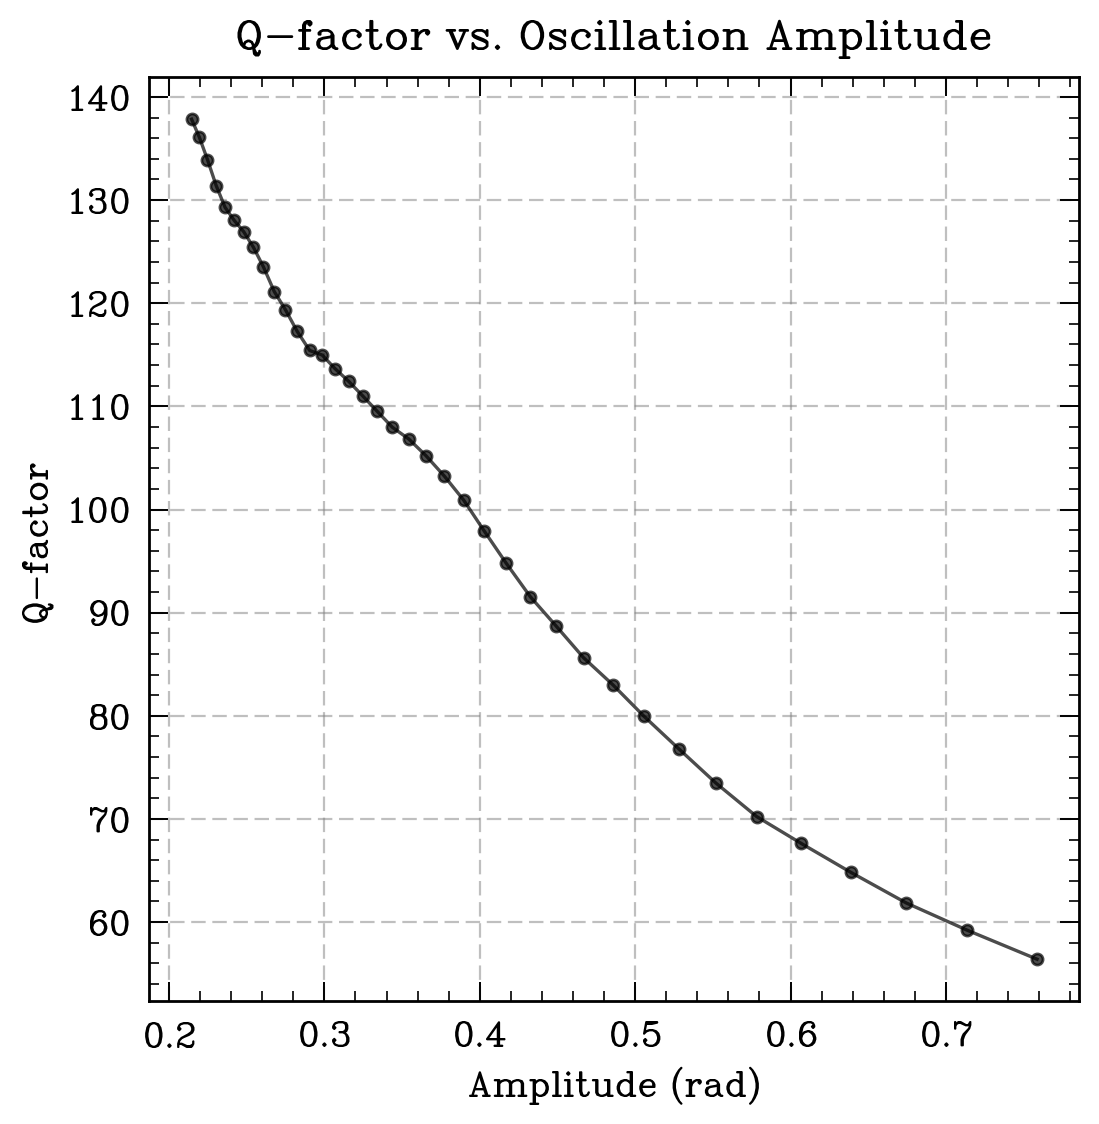
\includegraphics[width=0.8\linewidth]{q_amplitude.png}
    \label{fig:q_amp}
    \caption{Plot of pendulum period against oscillation amplitude. Datapoint errorbars are calculated using standard deviation ($\epsilon = 1\sigma$). $\theta$ referenced in the legend is the transient amplitude of oscillation.}
\end{figure}
\begin{figure}[htb]
    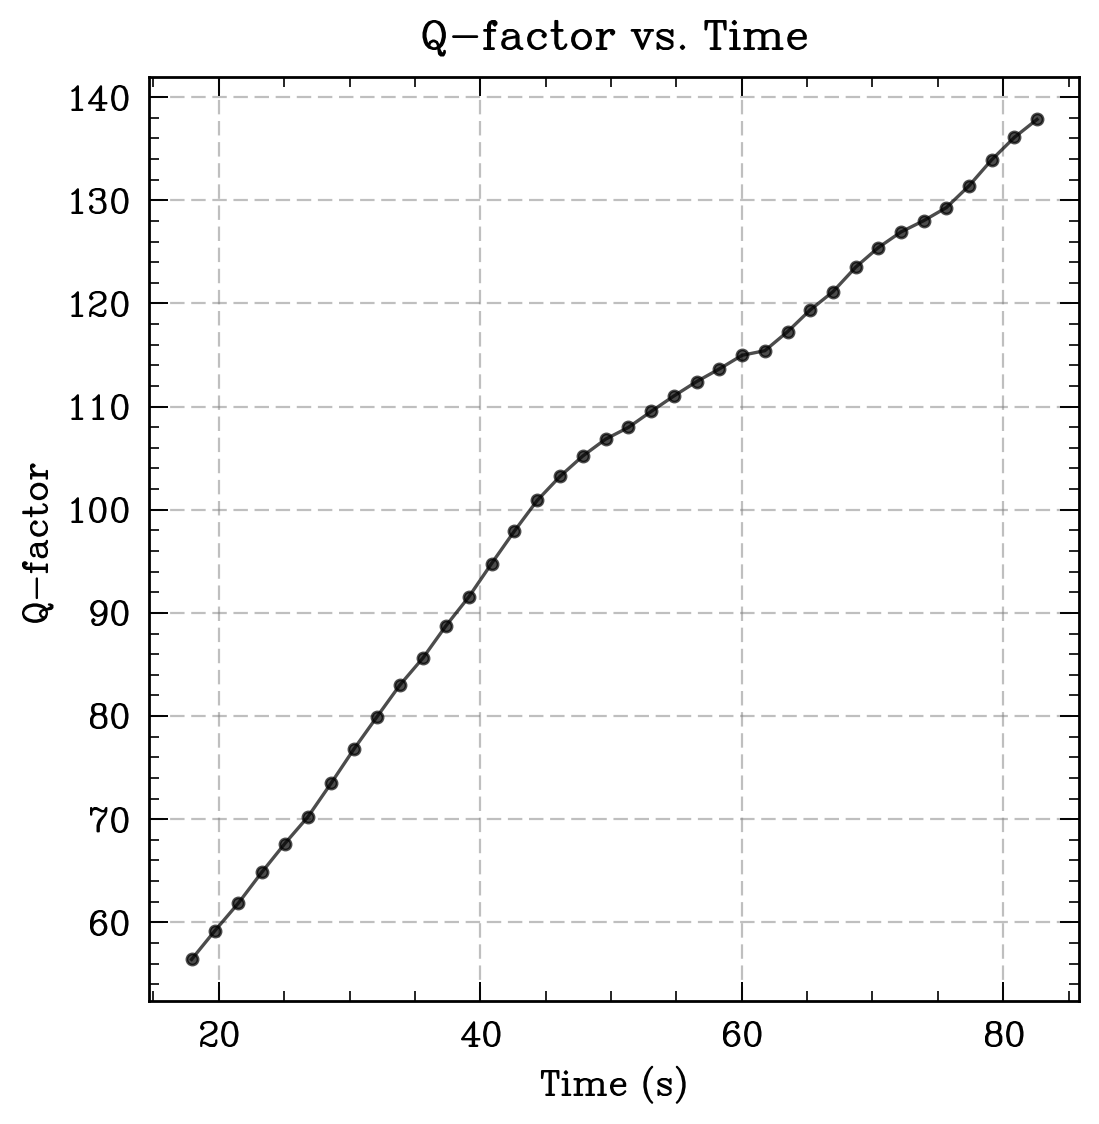
\includegraphics[width=0.8\linewidth]{q-time.png}
    \label{fig:q_time}
    \caption{Plot of pendulum period against oscillation amplitude. Datapoint errorbars are calculated using standard deviation ($\epsilon = 1\sigma$). $\theta$ referenced in the legend is the transient amplitude of oscillation.}
\end{figure}


\section{Conclusion}
In this report, we investigated the motion of a suspended magnet under the influence of attractive magnets placed on a base.


\onecolumngrid
\newpage

\section{References}

Wilson, Brian, “PHY180 Pendulum Project”, from
\href{https://q.utoronto.ca/courses/411727/files/39071655?module_item_id=7122439}{q.utoronto.ca}, 2025.

\section{Appendix}
Hellloooooooooo

\subsection{Out-of-plane Oscillations}
\bibliography{refs.bib}{}
\bibliographystyle{plain}
\end{document}
